\documentclass{beamer}

\usepackage[T1]{fontenc}
\usepackage[utf8]{inputenc}
\usepackage[french]{babel}
%\frenchbsetup{StandardLists=true}
%\usepackage{enumitem}
\usepackage{graphicx}
\usepackage{setspace}
%\usepackage{mathabx}
%\usepackage{eurosym}
%\usepackage{xstring}
\usepackage{textcomp}

%%% MACRO %%%


% FIXME Prendre en compte les majuscule déjà présente
\makeatletter
\@ifpackageloaded{xstring}{
	\newcommand\smallcaps[1]{\StrLeft{#1}{1}\scriptsize\uppercase{\StrGobbleLeft{#1}{1}}\normalsize }
}{
	\newcommand\smallcaps[1]{\textsc{#1}}
}
\makeatother



%===============================================================================
% Définit un type de puce pour une liste. Si le pakage "pifont" est chargé, il 
% est utilisé, sinon on met un tiret.
\makeatletter
\@ifpackageloaded{pifont}{
	\newcommand\goodItemArrow[0]{\ding{226}}
}{
	\newcommand\goodItemArrow[0]{-}
}
\makeatother



%===============================================================================
% Item de liste avec spécification de la puce et paramètre écrit en gras.
\newcommand\functionality[1]{
	\item[\goodItemArrow] \textbf{#1}\\
}



%===============================================================================
% Commande \Euro indépendante des paquets chargés 
\makeatletter
\@ifpackageloaded{eurosym}{
	\newcommand\Euro[0]{\euro{}}
}{
	\@ifpackageloaded{textcomp}{
		\newcommand\Euro[0]{\texteuro}
	}{
		\newcommand\Euro[0]{Euro}
	}
}
\makeatother



%===============================================================================
% Accès à des variables dans le document. 
%\makeatletter
%\let\titleName\@title
%\let\subtitleName\@subtitle
%\let\authorName\@author
%\makeatother



% Titre de la section courante (que dans beamer)
%\secname 
% Titre de la sous-section courante (que dans beamer)
%\subsecname




\title[Réunion GO/NO GO]{Surfaces de révolution discrètes}
%\author[\smallcaps{Ben Othmane} Zied \\\smallcaps{Benoist} Thomas \\\smallcaps{Bisutti} Adrien \\\smallcaps{Richaume} Lydie]{BEN OTHMANE Zied \\BENOIST Thomas \\BISUTTI Adrien \\RICHAUME Lydie} % FIXME Enlever les parenthèses
\institute{Université de Poitiers}
\date{15 octobre 2015}

\usetheme{Madrid}
%\usetheme{JuanLesPins}
\usecolortheme{sidebartab}
\usefonttheme{professionalfonts}
%\useinnertheme{nom du theme interne}
%\useoutertheme{nom du theme externe}



% Changement du tempplate de base ----------------------------------------------
\AtBeginSection[]{
	\begin{frame}{Plan}
	  	\tableofcontents[currentsection, hideothersubsections]
	\end{frame}
}

%\defbeamertemplate*{title page}{customized}[1][]
%{
%  \usebeamerfont{title}\inserttitle\par
%  \usebeamerfont{subtitle}\usebeamercolor[fg]{subtitle}\insertsubtitle\par
%  \bigskip
%  \usebeamerfont{author}\insertauthor\par
%  \usebeamerfont{institute}\insertinstitute\par
%  \usebeamerfont{date}\insertdate\par
%  \usebeamercolor[fg]{titlegraphic}\inserttitlegraphic
%}

% nouvelle commande ------------------------------------------------------------
%\newcommand\smallcaps[1]{
%	\uppercase{\StrChar{#1}{1}}
%%	\StrDel[1]{#1}{\StrChar{#1}{1}}
%%	\small{\uppercase{\bsuffix}}

%}
\definecolor{titlecolor}{RGB}{51, 51, 179}
\newenvironment<>{titleblock}[1]{%
	\setbeamercolor{block body}{fg=white, bg=titlecolor}%
	\begin{block}#2{#1}}{\end{block}}
\begin{document}

%\begin{frame}{test}
%%	\StrDel[1]{azerty}{\StrChar{azerty}{1}}
%	\StrChar{azerty}{1}\\
%	\StrBefore{azerty}{z}
%\end{frame}

%===============================================================================
%	TITRE
%===============================================================================
\begin{frame}
	\titlepage
	% FIXME inseré logo
	
\includegraphics[width=2cm]{../Images/logo-Xlim.png}
	\hfill
	
\includegraphics[width=2cm]{../Images/logo_univ_poitiers.png}
\end{frame}


%===============================================================================
%	PLAN
%===============================================================================
\begin{frame}{Plan}
	\tableofcontents[hidesubsection]
\end{frame}


%===============================================================================
%	INTRODUCTION
%===============================================================================
\section{Introduction}
	\begin{frame}{Participants}
		\begin{itemize}
			\item Clients~:\\
				\begin{itemize}
					\item Éric \smallcaps{Andres} (Professeur et Directeur de département XLIM-SIC)
					\item Gaëlle \smallcaps{Largeteau-Skapin} (Maitre de Conférence,Géométrie~discrète)
				\end{itemize}
			\item Exemple d'utilisateur final~:
				\begin{itemize}
					\item Aurélie \textsc{Mourier} (Artiste)
				\end{itemize}
			\item Encadrant pédagogique~: 
				\begin{itemize}
					\item Philippe \textsc{Meseure} (Professeur, Informatique graphique)
				\end{itemize}
		\end{itemize}
		\begin{itemize}
			\item Composition de l'équipe~:
				\begin{itemize}
					\item Zied \textsc{Ben Othmane}
					\item Thomas \textsc{Benoist}
					\item Adrien \textsc{Bisutti} %(Gestion des riques)
					\item Lydie \textsc{Richaume}
				\end{itemize}
		\end{itemize}
	\end{frame}


%===============================================================================
%	Projet
%===============================================================================
\section{Projet}


% --- Contexte -----------------------------------------------------------------
	\subsection{Contexte}
		\begin{frame}{Contexte}
			\begin{itemize}
				\item Nouvel algorithme conçu par Éric \textsc{Andres} et Gaëlle \textsc{Largeteau-Skapin} pour modéliser des surfaces de révolution~discrètes.
				\item Résultats actuellement modélisés sur Mathématica.
			\end{itemize}
			\begin{figure}
				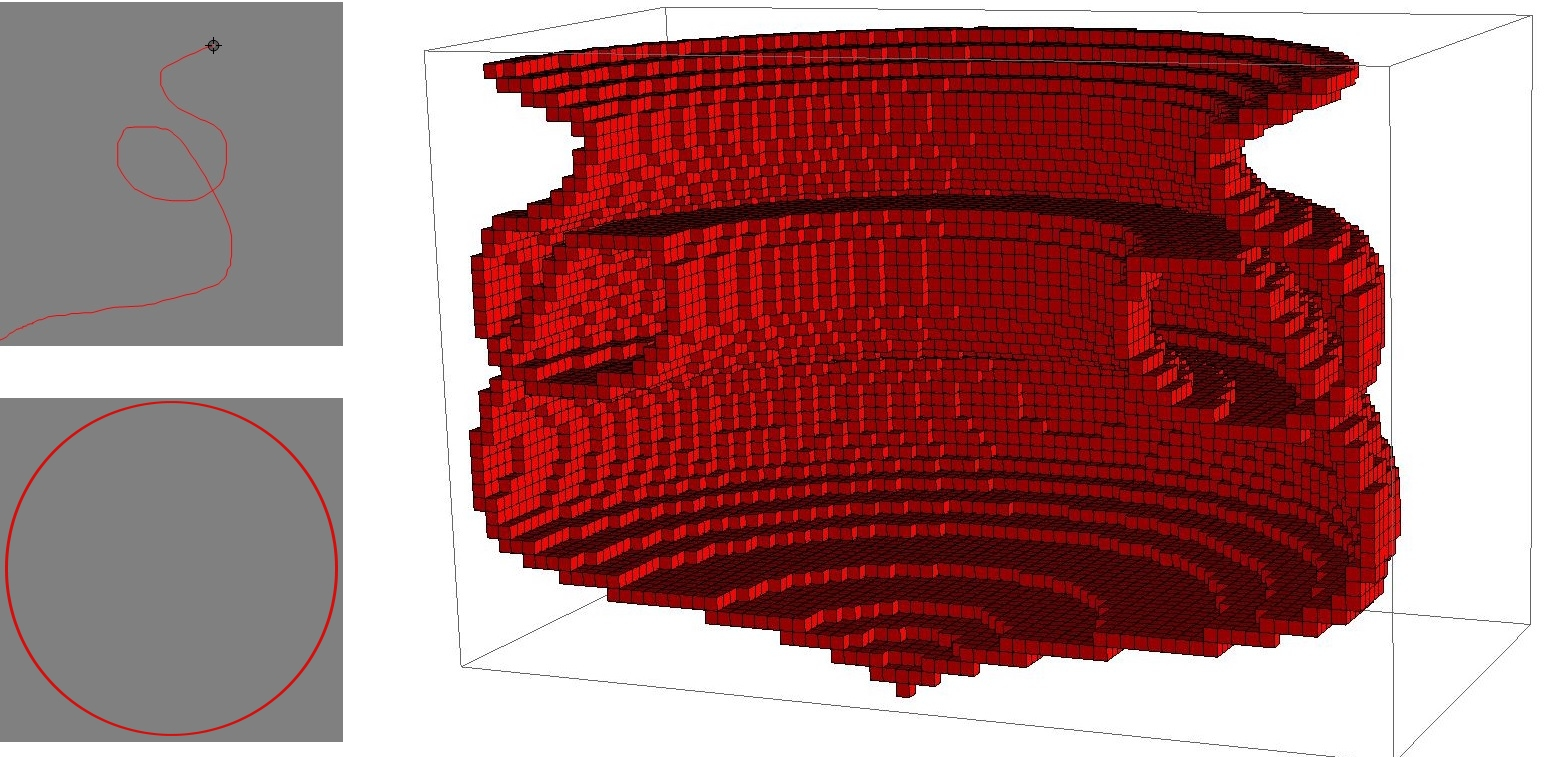
\includegraphics[height=3.8cm]{../Images/revolution2.jpg}
			\end{figure}
			\begin{itemize}
				\item[$\to$] Besoin de montrer les résultats et d'avoir un outil de création de surfaces de révolutions : but scientifique et artistique
			\end{itemize}
		\end{frame}


% --- Objectifs ----------------------------------------------------------------
	\subsection{Objectifs}
		\begin{frame}{Objectifs}
			\begin{itemize}
%				\item Développer un outil de visualisation des surfaces obtenues sous forme d'une application web % illustrant les résultats de l'algorithme
				\item Outil de visualisation de surfaces
					\begin{itemize}
						\item Visualiser en 3D, en coupe
						\item Choisir les médianes et les courbes de révolution
				 		\item Exporter des objets obtenus
					\end{itemize}
			\end{itemize}
			\begin{itemize}
				\item Algorithme de construction des surfaces de révolution
					\begin{itemize}
						\item Fourni par les clients
						\item Possibilité d'évolution de l'algorithme
					\end{itemize}
			\end{itemize}
		\end{frame}


% --- Containtes----------------------------------------------------------------
		\begin{frame}{Contraintes}
		\subsection{Contraintes}
			\begin{itemize}
%				\item Contraintes
%					\begin{itemize}
				\item Application pour le web
%						\item Deux types d'utilisateurs (scientifiques, et autres)
%					\end{itemize}
			\end {itemize}
			\begin{itemize}
				\item Accessible pour tout type d'utilisateur
					\begin{itemize}
						\item Utilisateurs lambda : Paramètres simples, formes prédéfinies, tracé à main levée
						\item Utilisateurs avancés : Contrôle plus précis
					\end{itemize}
			\end{itemize}
		\end{frame}


%===============================================================================
%	SOLUTION
%===============================================================================
\section{Propositions de solutions}


% --- Techno envisagées --------------------------------------------------------
	\subsection{Technologies envisagées}
		\begin{frame}{Technologies envisagés}
			\begin{itemize}
				\item Mathématica ?
					\begin{itemize}
						\item[$\oplus$] Réutilisation du code fourni par Éric Andres
						\item[$\ominus$] Application client $\to$ achat de la licence
						\item[$\ominus$] Application serveur $\to$ pas de serveurs
					\end{itemize}
			\end{itemize}
			\begin{itemize}
				\item HTML5 canvas / Javascript WebGL
					\begin{itemize}
						\item Technologie Web
						\item Maitrisés par la plupart des membres de notre équipe
						\item Participation à un projet similaire
					\end{itemize}
			\end{itemize}
		\end{frame}


% --- Réutilisation Bifurcations -----------------------------------------------
	\subsection{Réutilisation de l'existant}
		\begin{frame}{Réutilisation de l'existant}
			\begin{figure}
				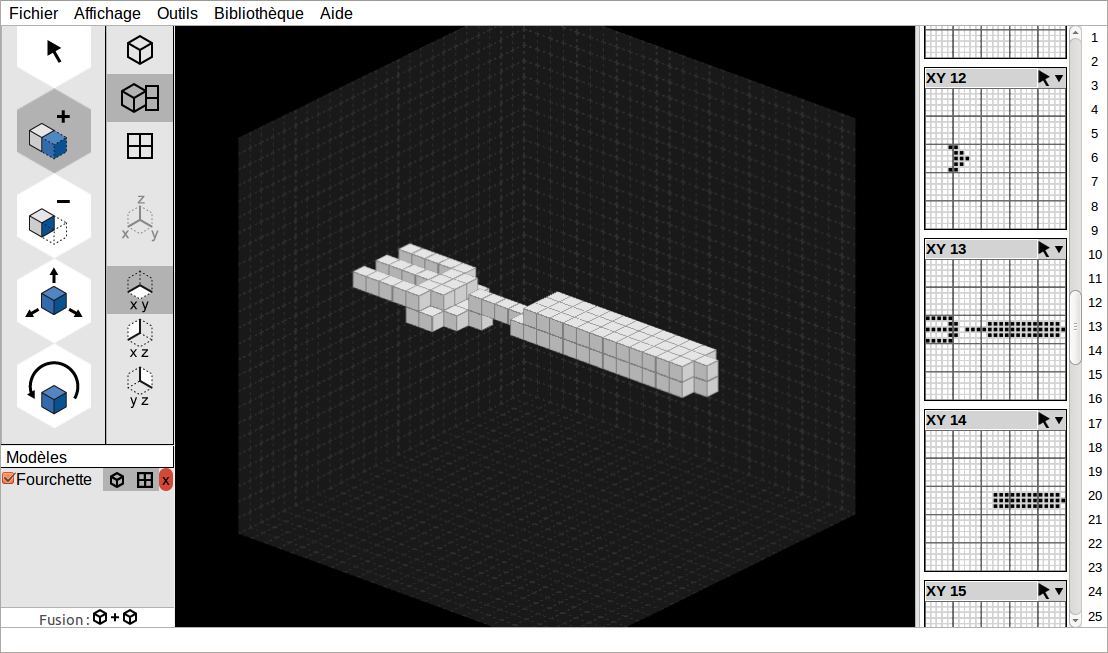
\includegraphics[width=12cm]{../Images/bifurcations_ihm.png}
			\end{figure}
		\end{frame}


% --- Interface et scénario ----------------------------------------------------
	\subsection{Proposition d'interface}
		\begin{frame}{Proposition d'interface}
			\begin{figure}
				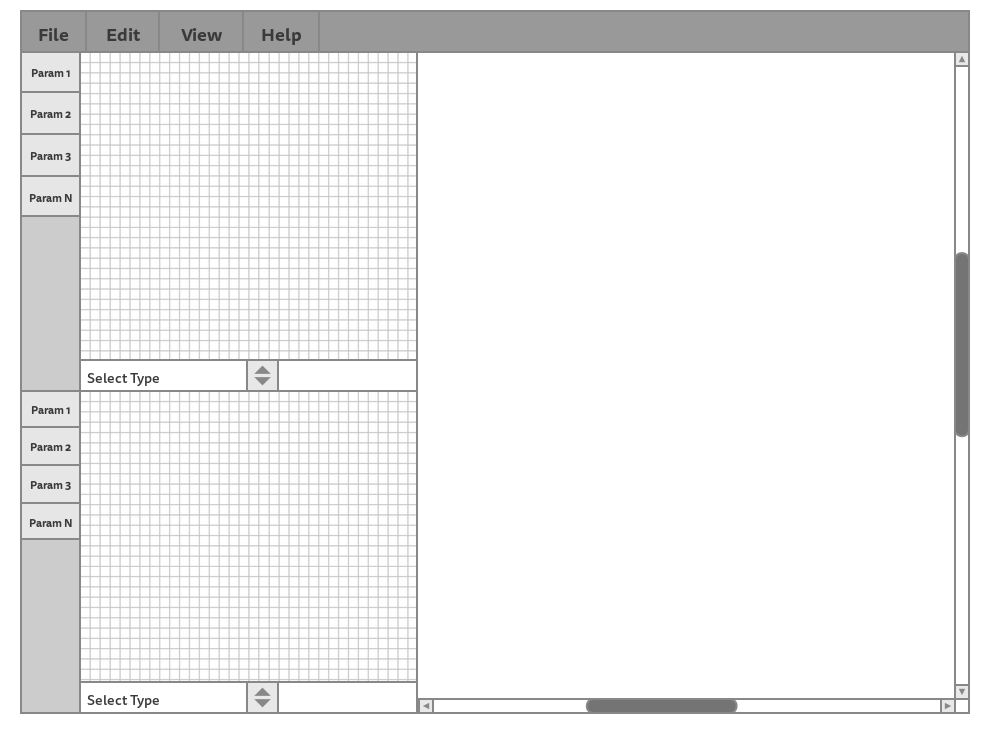
\includegraphics[width=10cm]{../Images/example_ihm.png}
			\end{figure}
		\end{frame}

		\begin{frame}{Proposition d'interface}
			\begin{figure}
				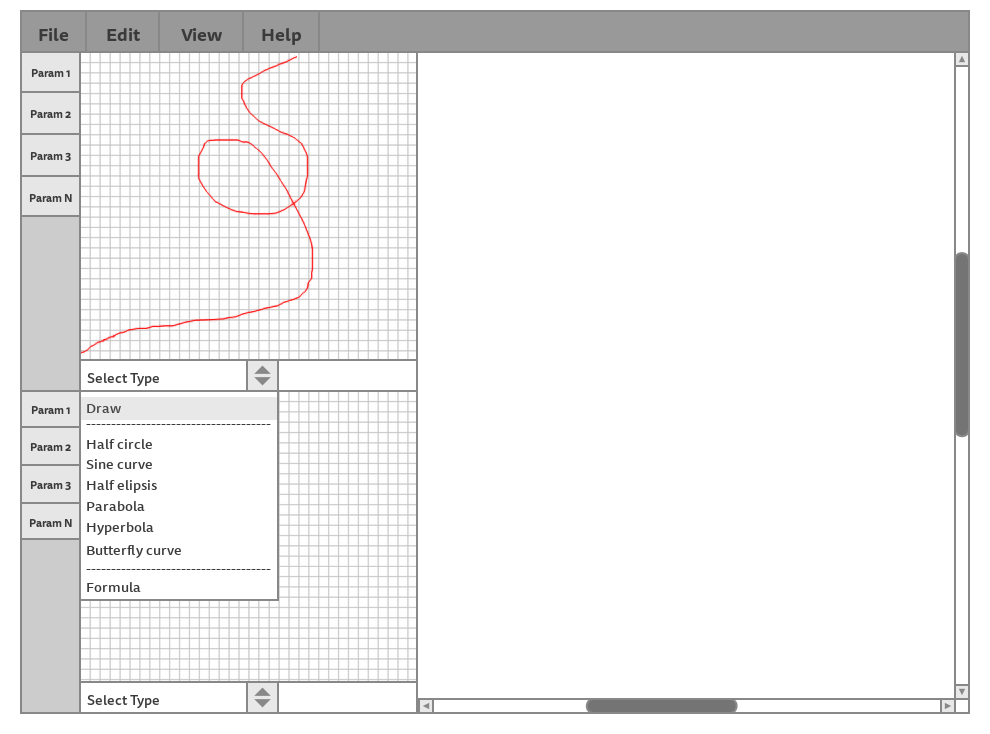
\includegraphics[width=10cm]{example_ihm_2.png}
			\end{figure}
		\end{frame}

		\begin{frame}{Proposition d'interface}
			\begin{figure}
				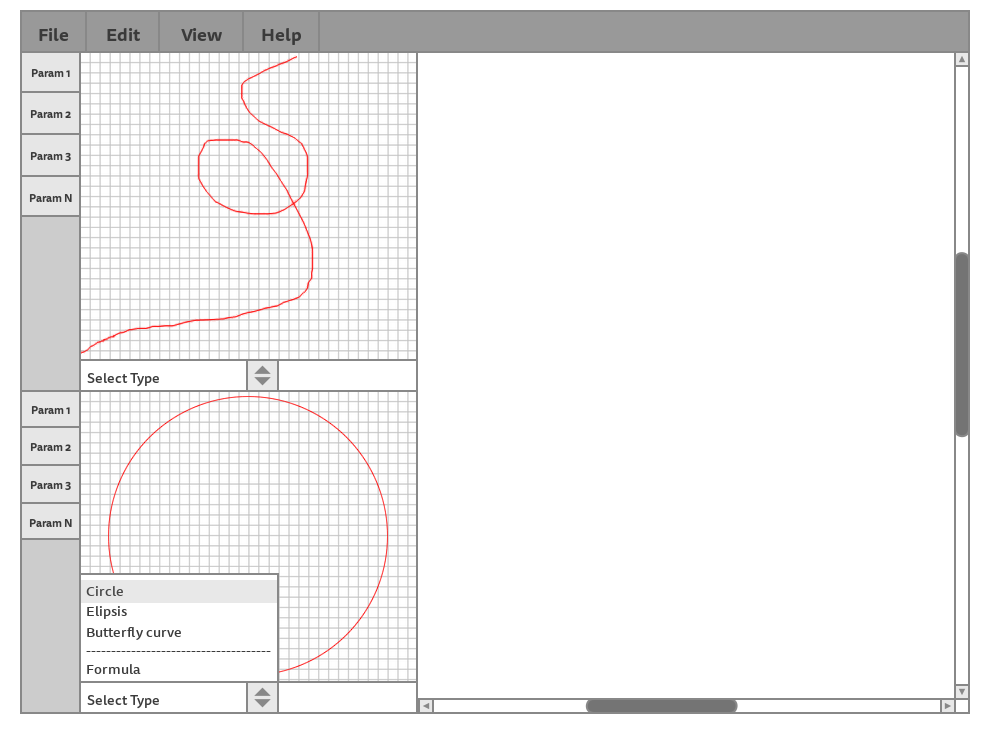
\includegraphics[width=10cm]{example_ihm_3.png}
			\end{figure}
		\end{frame}

		\begin{frame}{Proposition d'interface}
			\begin{figure}
				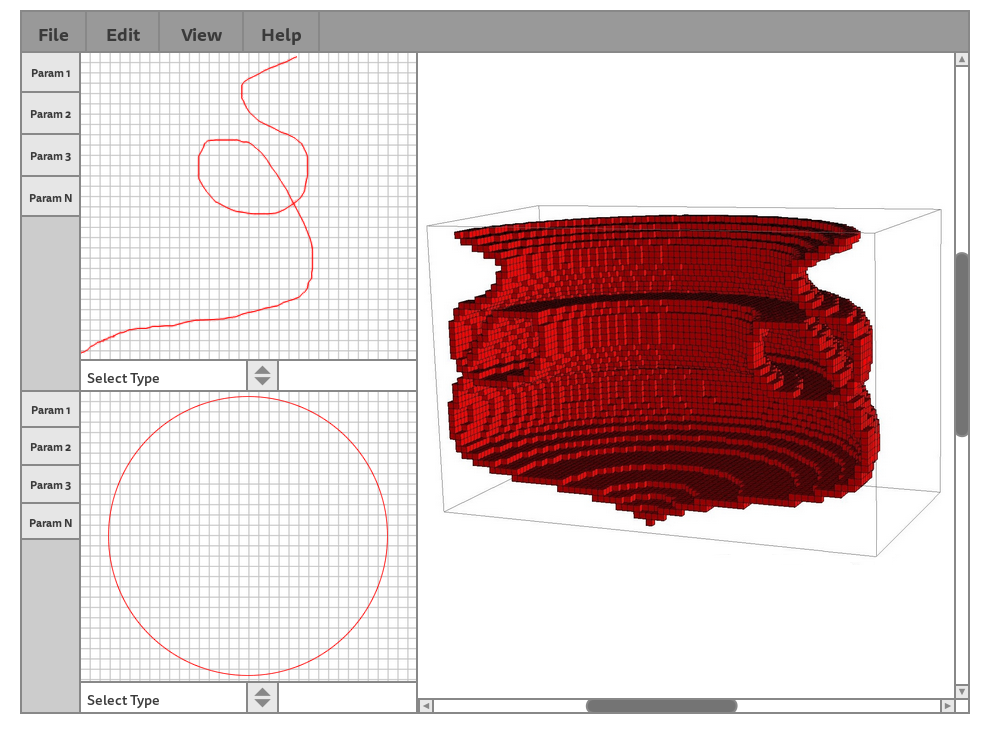
\includegraphics[width=10cm]{example_ihm_4.png}
			\end{figure}
		\end{frame}

% --- Récapitulitif du scénario ------------------------------------------------
		\begin{frame}{Proposition d'interface}
			\begin{itemize}
				\item Choix de la méridienne~:
					\begin{itemize}
						\item Formes prédéfinies
						\item Option ``Tracé à main levée''
						\item Option ``Entrer une formule'' (facultative)
					\end{itemize}
			\end{itemize}
			\begin{itemize}
				\item Choix de la courbe de révolution~:
					\begin{itemize}
						\item Formes prédéfinies
						\item Option ``Entrer une formule'' (facultative)
					\end{itemize}
			\end{itemize}
%			\begin{itemize}
%				\item Génération de la surface par l'utilisateur
%			\end{itemize}
		\end{frame}


%===============================================================================
%	CONDUITE DE PROJET
%===============================================================================
\section{Conduite de projet}
	\subsection{Gestion de projet}
		\begin{frame}{Gestion de projet}
			\begin{itemize}
				\item Développement en spirale
					\begin{itemize}
						\item Application minimale fonctionnelle
						\item Adapté à notre emploi du temps
						\item Jalons de validation de l'interface par les clients
					\end{itemize}
			\end{itemize}
			\begin{itemize}
				\item Tâches importantes
					\begin{itemize}
						\item Refactoring du code du projet "Bifurcations"
						\item Design de l'interface
						\item Transcription de l'algorithme
						\item Amélioration de la vitesse de rendu
%						\item Tests régulier de l'interface
					\end{itemize}
			\end{itemize}
		\end{frame}

	
% --- Risques ------------------------------------------------------------------
	\subsection{Risques}
		\begin{frame}{Risques}
			\begin{itemize}
				\item Rendu 3D demandant trop de ressources 
				\item Interface à réaliser pour deux catégories d'utilisateurs
				\item Panne de matériel, problème logiciel, etc.
				\item Absence prolongée d'un des membres de l'équipe
			\end{itemize}
		\end{frame}

	
% --- Cout ---------------------------------------------------------------------
	\subsection{Coûts}
		\begin{frame}{Coûts}
			\begin{itemize}
				\item Jeune ingénieur~: 3 000 \Euro / mois
				\item 4 personnes pendant 10 semaines
				\item Coût de revient~: 30 000 \Euro 
				\item Prix proposé~: 40 000 \Euro
			\end{itemize}
		\end{frame}

%===============================================================================
%	CONCLUSION
%===============================================================================
\section{Conclusion}
	\begin{frame}{Conclusion}
		\begin{itemize}
			\item Application de génération de surfaces de révolution
				\begin{itemize}
					\item Application web destinée à plusieurs types d'utilisateurs
					\item Utilisation de l'application pour montrer les résultats de la publication
				\end{itemize}
			\item Prochaines étapes~:
				\begin{itemize}
					\item Pré-étude du projet (format d'export, amélioration de l'algorithme de~rendu)
					\item Propositions de solutions pour l'interface multi-profiles
				\end{itemize}
		\end{itemize}
	\end{frame}


% --- Remerciment --------------------------------------------------------------
	\begin{frame}{}
		\bigskip
		\bigskip
		\begin{titleblock}{}
			\begin{center}
				\smallskip
				\Large Surfaces de révolution discrètes
				\smallskip
			\end{center}
		\end{titleblock}

		\bigskip
		\begin{center}
			Merci de votre attention.\\
			\medskip
			Avez-vous des questions\,?			
		\end{center}

		\bigskip
		\bigskip
		
\includegraphics[width=2cm]{../Images/logo-Xlim.png}
		\hfill
		
\includegraphics[width=2cm]{../Images/logo_univ_poitiers.png}
	\end{frame}

\end{document}


